\section{DETAILED DESIGN AND REALIZATION}

AtlantikSolar (Fig. \ref{fig:AtlantikSolarCollage}) is a solar-powered Low-Altitude Long-Endurance(LALE) Unmanned Aerial Vehicle designed for perpetual flight at $\varphi=45°$ geographical latitude from April 21\textsuperscript{st} to August 21\textsuperscript{st}. It was designed and built at ETH Zurich. Although its design is mostly dictated by the requirement for low level-flight power consumption, it provides means to mount an advanced optical\&infrared sensor pod developed at ETH Zurich for use in autonomous search and rescue or industrial inspection missions. The airplane airframe characteristics are summarized in table \ref{tab:DetailedDesignParameters}. An overview over the airplane system topology is given in Fig. \ref{fig:AtlantikSolar_SystemOverview}.
%\begin{figure}[tb]
%    \centering
%    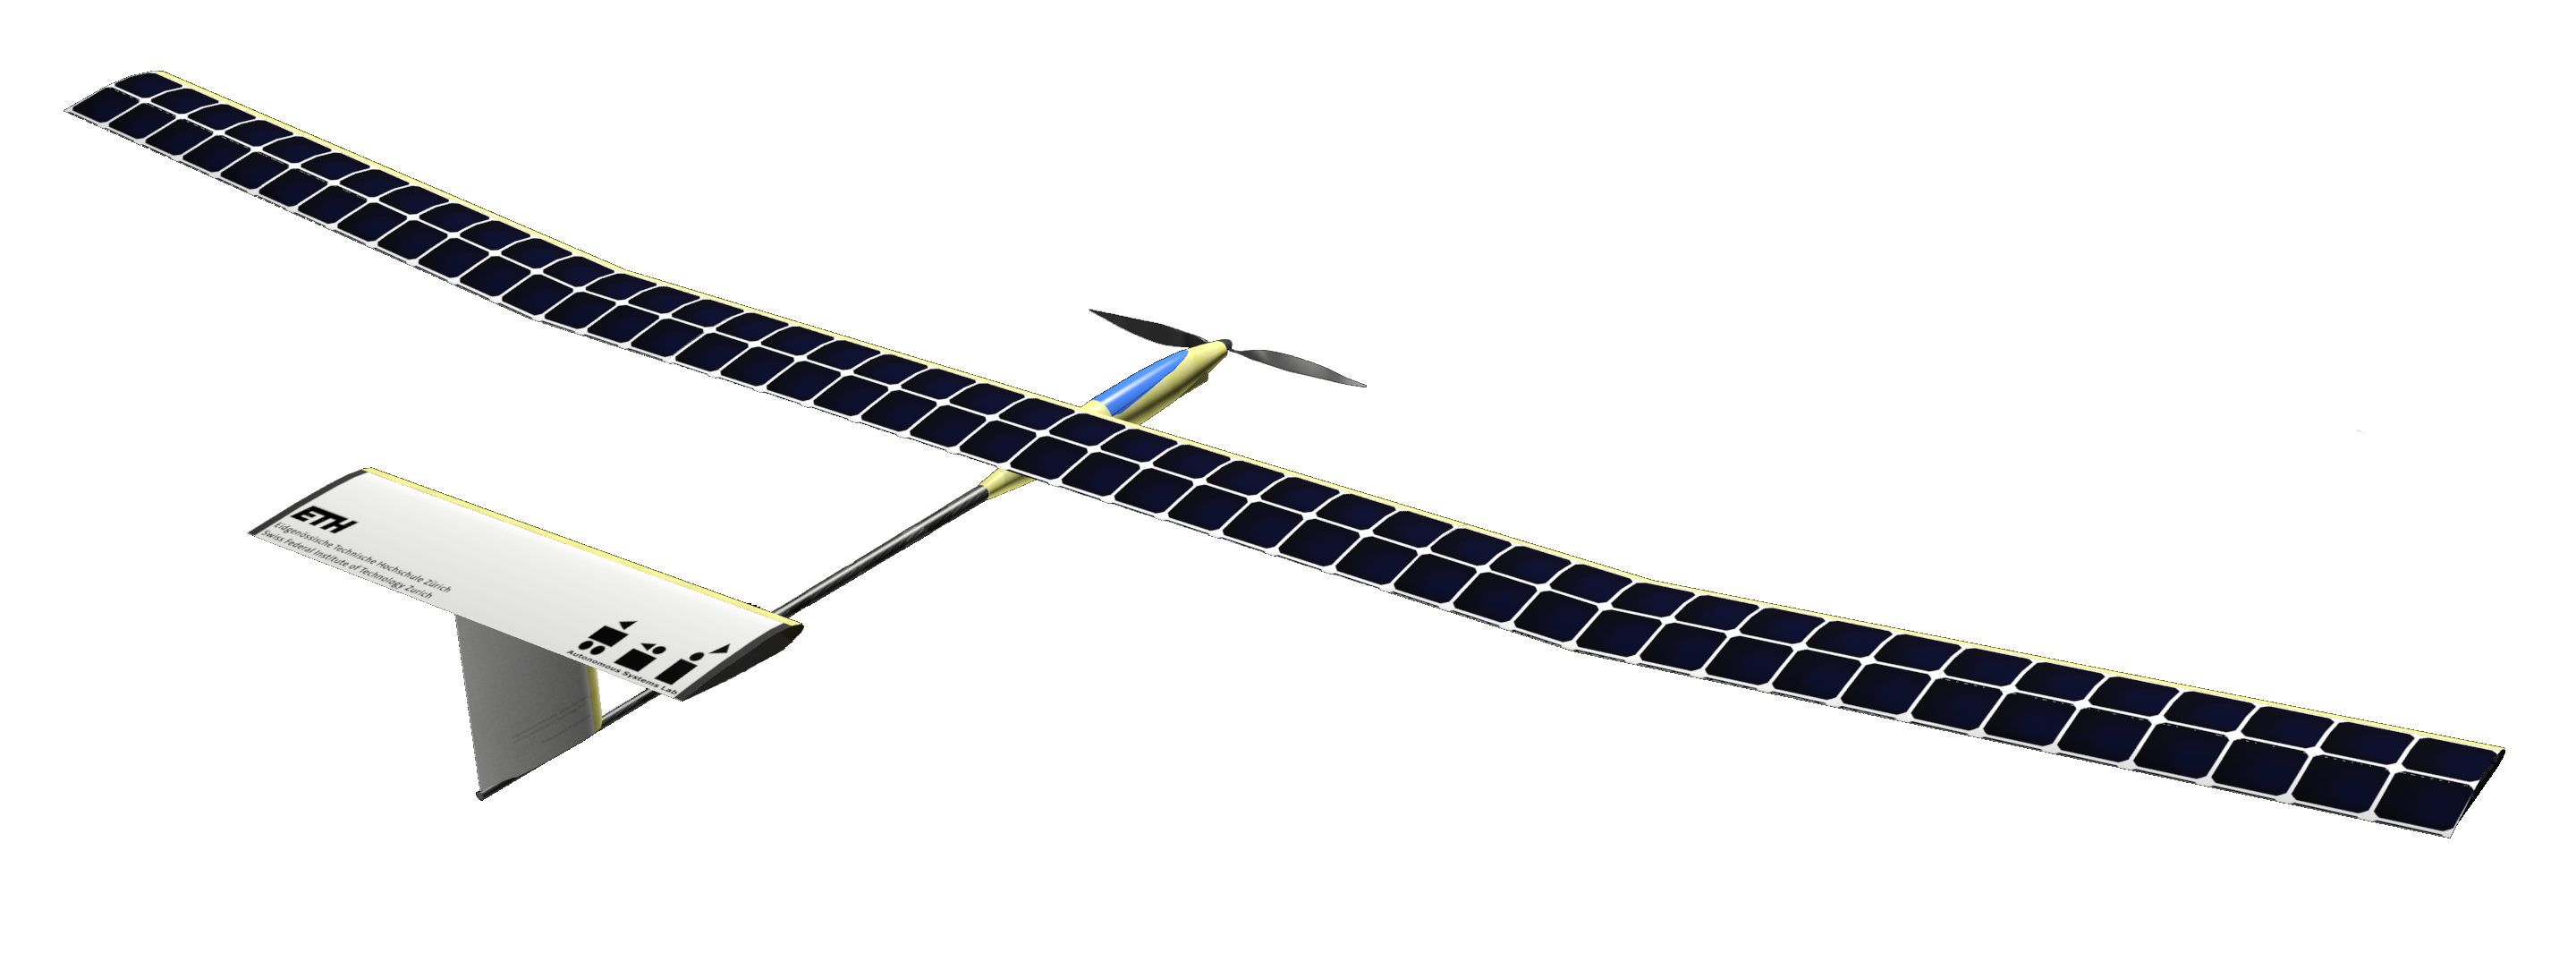
\includegraphics[width=\linewidth]{images/6_CAD_AtlantikSolarFull}
%    \caption{The AtlantikSolar UAV features a conventional T-tail configuration with 1 motor, two ailerons, an all-moving elevator and a rudder for actuation.}
%    \label{fig:CAD_AtlantikSolarFull}
%\end{figure}

\begin{table}
\caption{AtlantikSolar design characteristics}
\label{tab:DetailedDesignParameters}
\begin{center}
\begin{tabular}{l l}
Wing span & 5.65$\unit{m}$\\
\hline Wing chord& 0.305$\unit{m}$\\
\hline Length& 2.03\unit{m}\\
\hline Height&0.45\unit{m}\\
\hline Mass& 7.36$\unit{kg}$\\
\hline Battery mass& 3.52$\unit{kg}$\\
\hline Wing loading&4.28$\unitfrac{kg}{m^2}$\\
\hline Stall speed& 8.1$\unitfrac{m}{s}$\\
\end{tabular}
\end{center}
\end{table}

\subsection{UAV Platform Design}
\subsubsection{Airframe}
\label{secsec:Airframe and hardware}

The structure of AtlantikSolar is built in a traditional rib-spar construction method. The wing (Fig. \ref{fig:CAD_AtlantikSolarStructure}) consists of an inner cylindrical carbon-fibre spar to resist torsional wing loads. Four carbon-fibre belts of trapezoidal and laterally-varying cross-section are located around the spar to optimally resist bending loads and to provide maximum wing stiffness to protect the solar cells on the wings. Equally-spaced balsa-wood ribs and the kevlar-reinforced wing leading edge provide structural support for the non-load-carrying outer wing surface. The main wing is composed of the left, right and center wing and can be disassembled into three wing pieces of $b<2m$ each. The horizontal and vertical tail planes are constructed similar to the main wing.

\begin{figure}[tb]
    \centering
    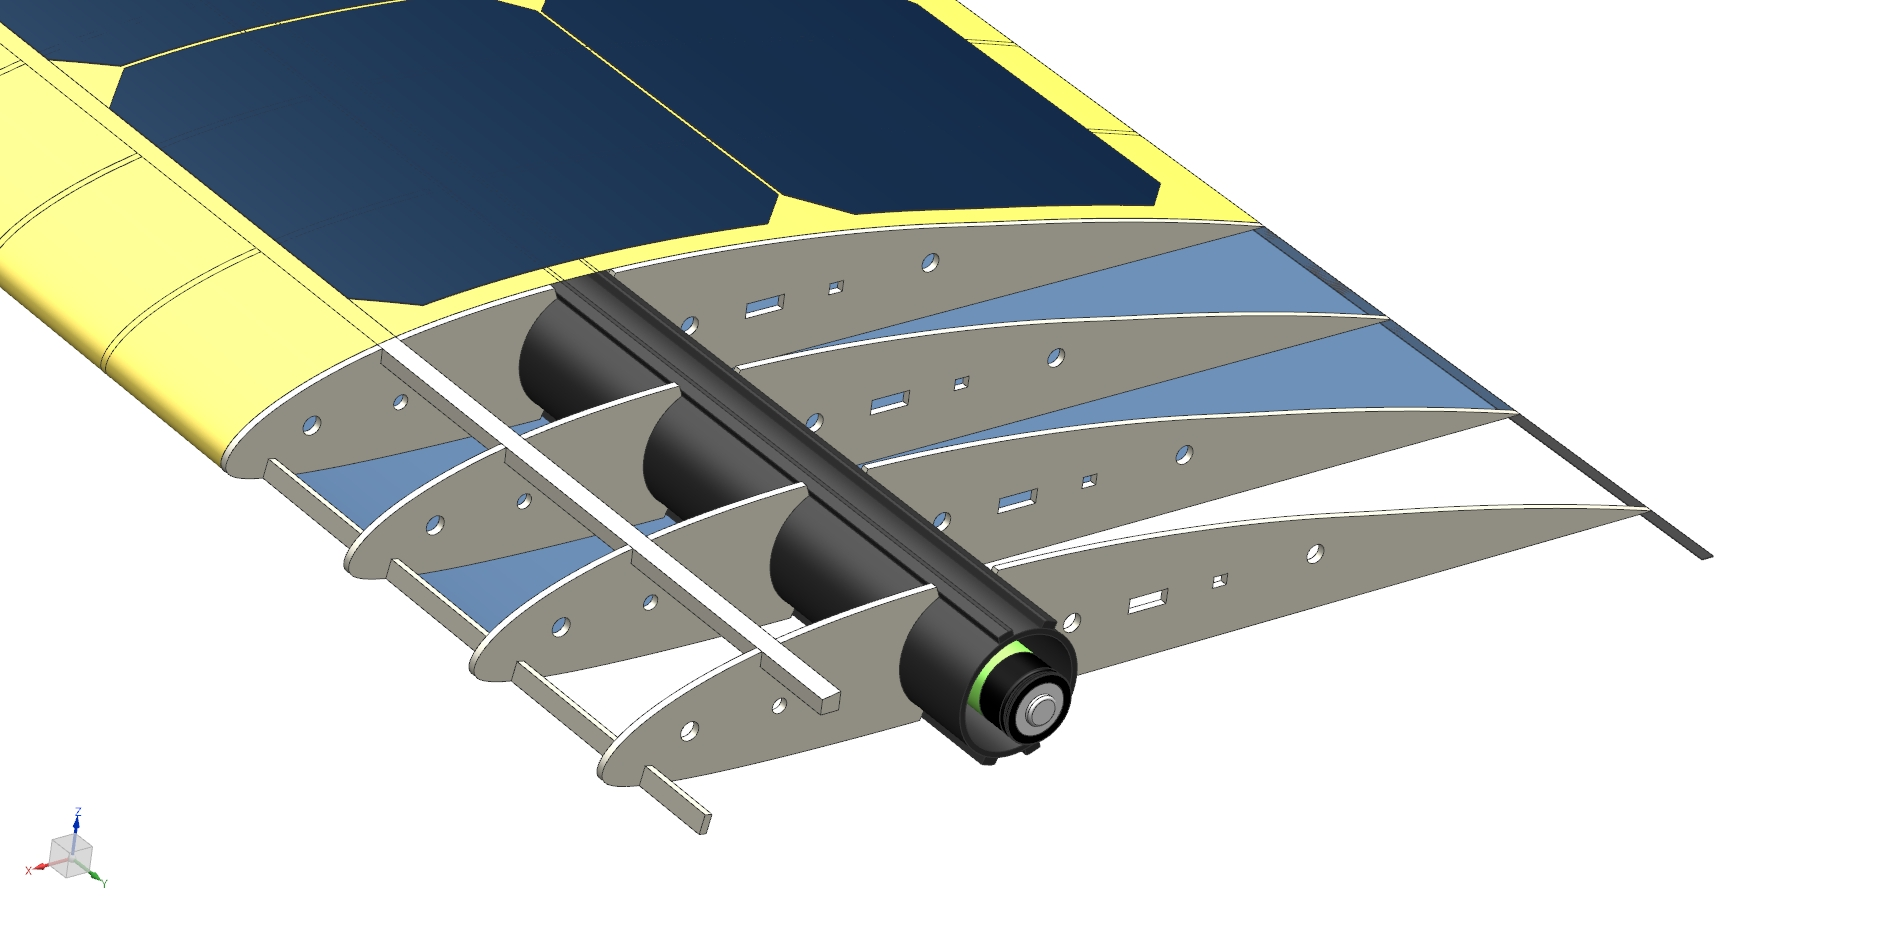
\includegraphics[width=\linewidth]{images/7_CAD_AtlantikSolarStructure}
    \caption{AtlantikSolar's wing structure, integrated batteries and solar cells.}
    \label{fig:CAD_AtlantikSolarStructure}
\end{figure}

\subsubsection{Energy Generation and Storage}
Depending on the application, the cylindrical wing spars are fitted with 60 to 72 cylindrical high energy-density industrial Lithium-Ion battery cells (Panasonic NCR18650b, 243Wh/kg) to optimally distribute the battery mass in a ``span loader'' concept. The cells are connected in a 6S (22.2V) configuration and provide $E_{bat,max}=850Wh$ at $m_{bat}=3.5kg$. The solar modules are seamlessly embedded into the upper wing surface to avoid premature flow separation. They feature a total of 88 SunPower C60 cells with a measured module-level efficiency of $\eta_{sm}=0.20$, an areal density of $k_{sm}=590g/m^2$ and a maximum power output of 275W at $\varphi=45°$ on June 21\textsuperscript{st}. Modules featuring SunPower E60 cells with a measured \cite{Sunier_EPFLSolarModules} module-level efficiency of $\eta_{sm}=0.23$ are currently being integrated.

\subsubsection{Actuation}
The propulsion system features a foldable custom built carbon-fibre propeller with diameter $D=66cm$ and pitch $H=60cm$. It is driven by a 5:1 reduction-ratio planetary gearbox, a RS-E Strecker 260.20 brushless DC motor with $k_V=570RPM/V$ and a Kontronik Koby 55 LV motor controller at up to $P_{prop,max}=450W$ electrical input power. The actuation system consists of four Volz DA-15N servos that drive the two ailerons, the all-moving elevator and the rudder. To guarantee reliable multi-day flight, the Volz actuators were successfully bench-tested throughout a simulated continuous 30-day flight \cite{DellaCa_BT}.
%mention wind tunnel, lab motor test stand tests? Only if space left...

\subsubsection{Avionics}
The AtlantikSolar avionics topology is shown in Fig. \ref{fig:AtlantikSolar_SystemOverview} and an integration snapshot is presented in Fig. \ref{fig:9_CAD_AtlantikSolarAvionics}. Multiple sensors are centered around a Pixhawk PX4 Autopilot - an open source and open hardware project initiated at ETH Zurich - with a Cortex M4F microprocessor running at 168Mhz and featuring 192kB RAM. For state estimation (Sec. \ref{secsec:StateEstimation}), an ADIS 16448 10-axis Inertial Measurement Unit (IMU), a u-Blox LEA-6H GPS receiver, and a Sensirion SDP600 differential pressure (i.e. airspeed) sensor are used. The SDP600 airspeed sensor has been chosen due to its low relative error of less than 5\% at airspeeds of 8m/s, which is necessary to closely control the airspeed to the airspeed with minimum required power $P_{out}$. Commands are received through a 433Mhz telemetry link for medium ranges, or through a long-range IRIDIUM-based satellite communication link that also serves as a backup in case of primary telemetry link failure. The airplane implements a fully manual RC-command fallback mode in case of a severe autopilot failure. Night operations are possible due to four on-board high-power position-indicating LEDs.

\begin{figure}[tb]
    \centering
     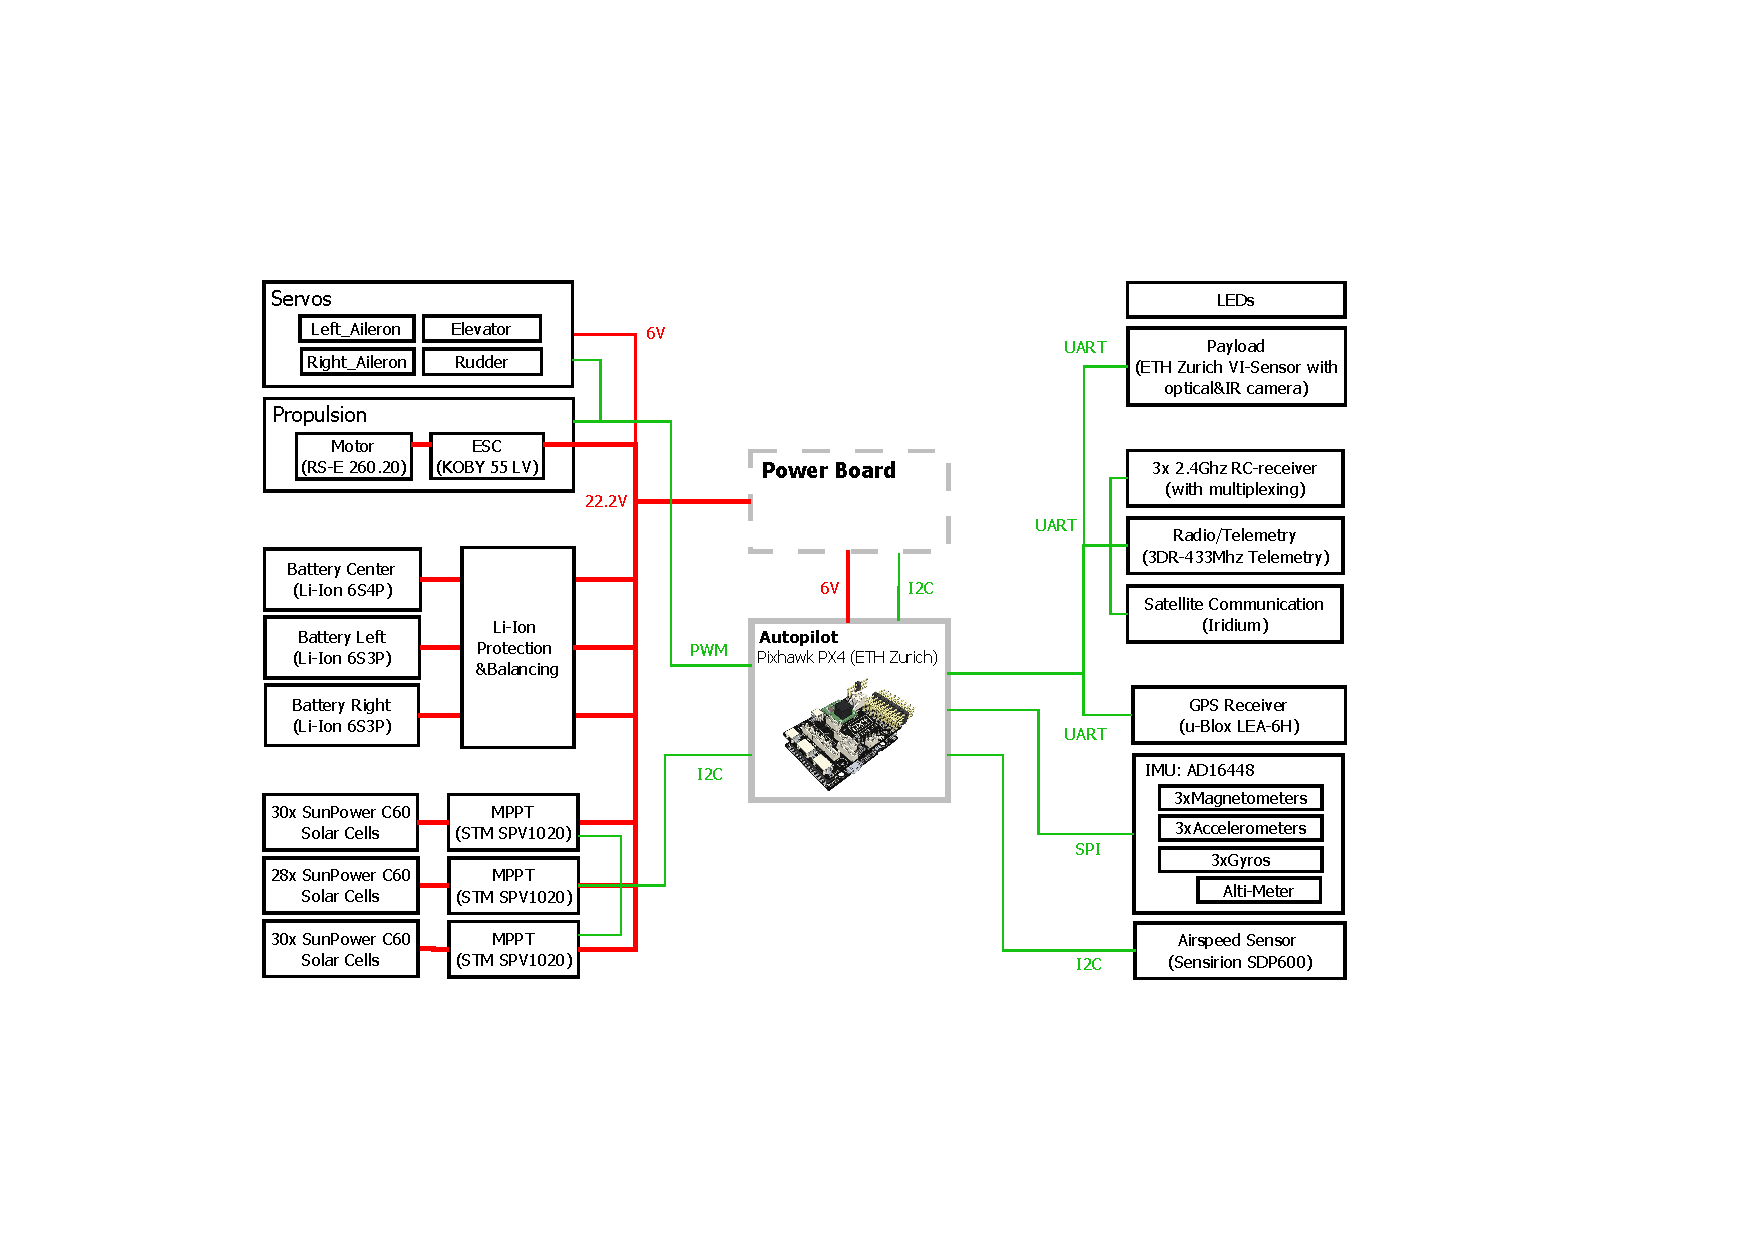
\includegraphics[width=\linewidth]{images/8b_AtlantikSolar_Avionics}
    \caption{AtlantikSolar system overview. For clarity, voltage lines from the autopilot to connected devices (5.0V and 3.3V) are omitted.}
    \label{fig:AtlantikSolar_SystemOverview}
\end{figure}

\begin{figure}[tb]
    \centering
    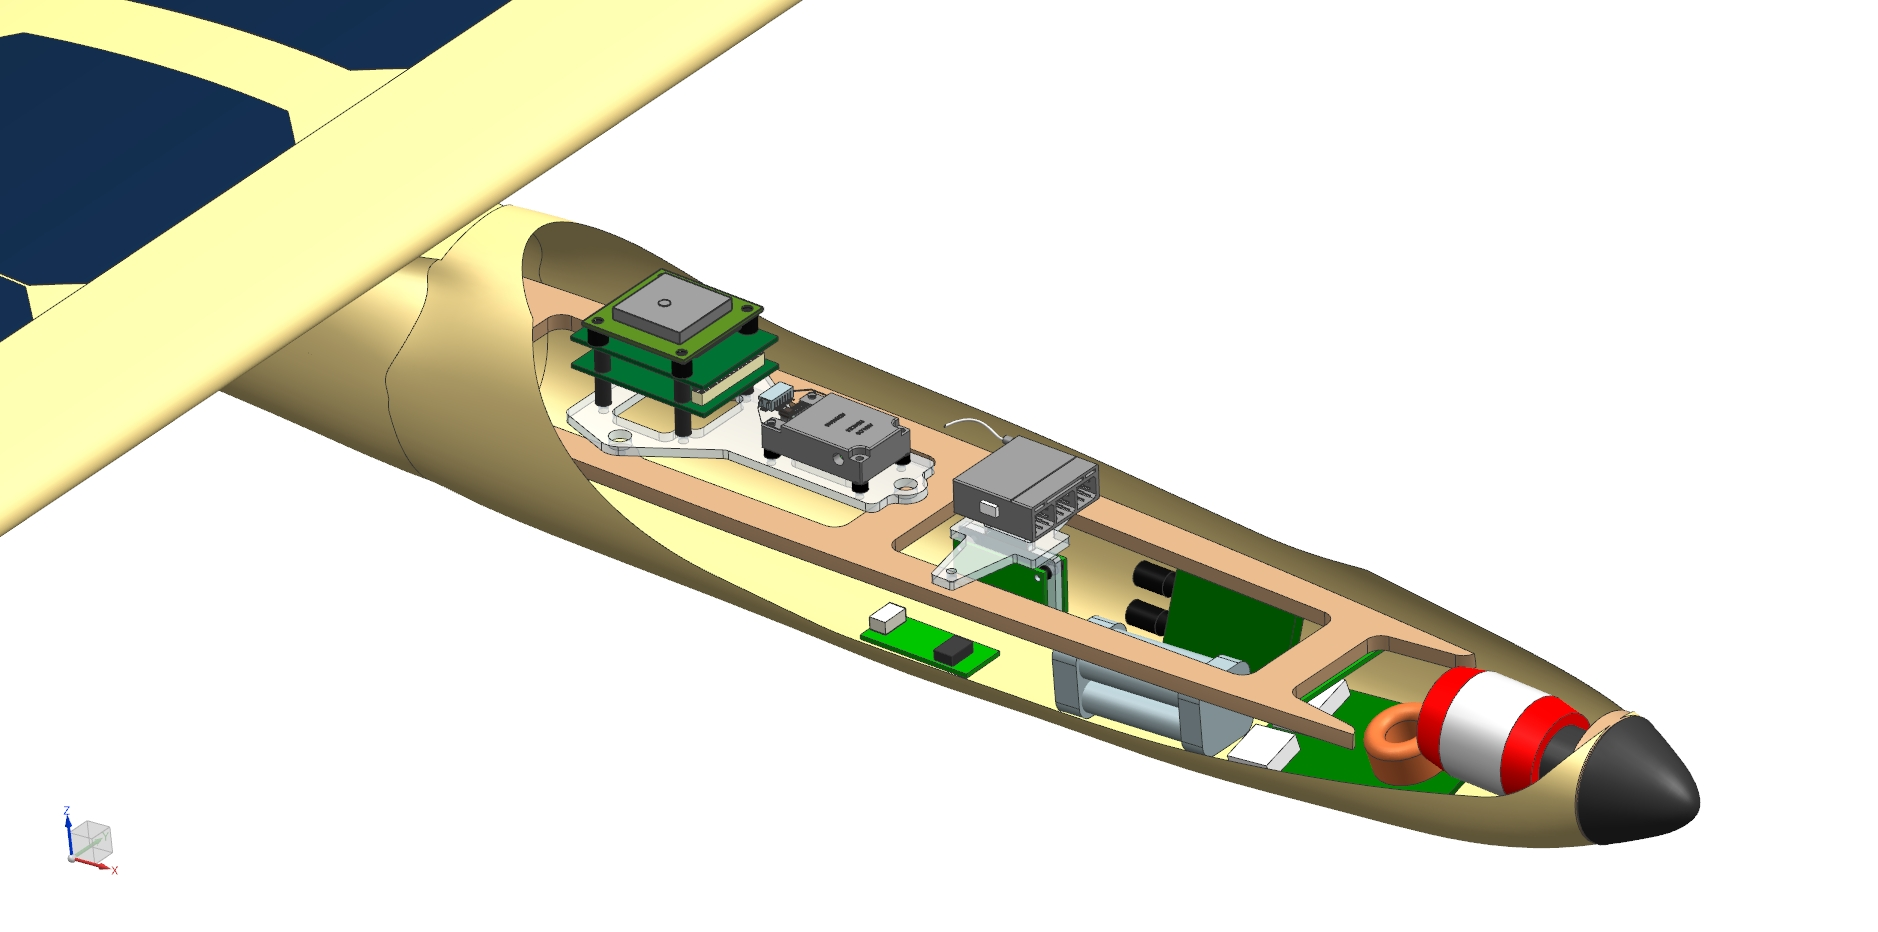
\includegraphics[width=\linewidth]{images/9_CAD_AtlantikSolarAvionics}
    \caption{Avionics components and their placement inside AtlantikSolar.}
    \label{fig:9_CAD_AtlantikSolarAvionics}
\end{figure}

\subsubsection{Payload}
% [THOMAS]
  - VI Sensor [ref to VI-sensor paper; ref to Leutenegger thesis?]
  - ~5 sentences + 1 picture
  
\subsection{State Estimation and Control Design}
Onboard state estimation \& control
\subsubsection{State Estimation}
\label{secsec:StateEstimation}
% [AMIR]
  - brief (5 sentence) description of SE type/principle
  - one verification plot (e.g. gps position ``ground truth'' vs. estimated position) 
  then REF to stefan\&Amir paper

\subsubsection{System Identification}
%[DR. ALEXIS]
 - System Identification \& Modelling
 
 \subsubsection{Control}
 %[PHILIPP writes this, DR. ALEXIS checks this]
 - Control using PID,  outer loops TECS \& L1 (Ref to OMLAS MED paper, also saying that there is future technologies which are being developed).
 - Full pre-flight verification in HIL before going into flight tests
 
